\subsection{Reflection of a pressure in a blood vessel}
\subsubsection{Aim}



In this section, one tries to model the reflection of a blood pressure wave (PW) in a blood vessel (BV) using transmission line theory. Reflections in BV's are mostly generated by alterations in the geometry of the BV. Here, we look at two specific cases (Figure \ref{fig:model}): (1) a vasoconstriction and (2) an aneurysm and a vasoconstriction. Furthermore, the BV itself is considered as ideal;  since one is only interested in the \textit{reflection} of the PW at the load, losses due to the BV itself can be neglected and only losses from the alteration of the geometry are considered (load). That is, the resistance of the blood vessel is much smaller than the load resistance: $R_{\text{BV}} << R_L$. 

\begin{figure}[h!]
\centering
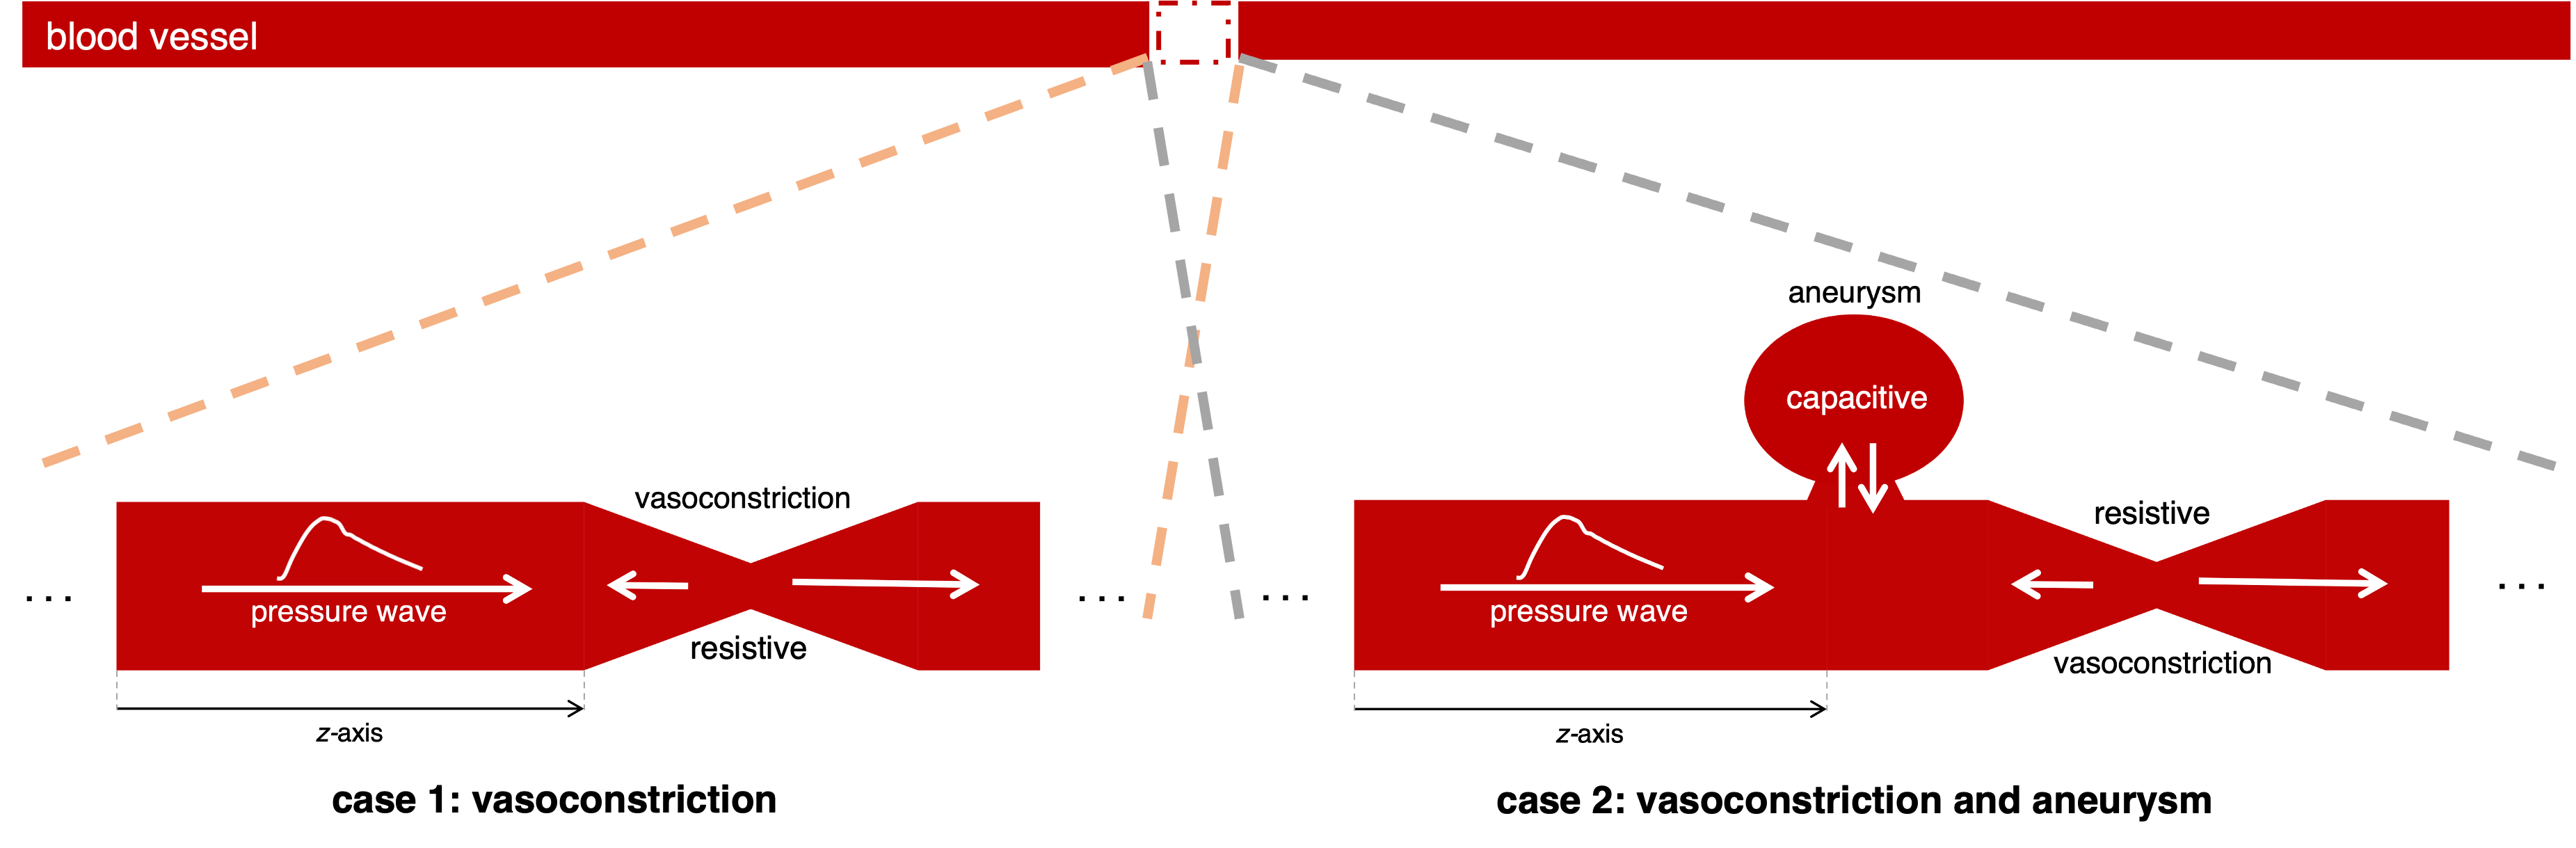
\includegraphics[width = \textwidth]{sum2.png}
\caption{Abstract drawing of cases to be modeled}\label{fig:model}
\end{figure}

\subsubsection{Implementation}
By analogy of Ohm's law, the relation of pressure $P$ and flow $Q$ is given by
\begin{equation}
P = RQ.
\end{equation}
Where $R$ is the resistance (medical units: mmHg/(ml/s)) the flow experiences. Here, its clear that $P$ takes the role of $V$ and $Q$ of $I$. The vasoconstriction in the BV hinders the flow to continue and thus can be treated as a resistor. In contrary, the aneurysm is able to store blood and can be interpreted as a capacitor.\\
 
Now, the implementation to the LTL model is obvious; we replace the source signal by  the incident PW: a 4$^{\text{th}}$ order windkessel blood pressure pulse\footnote{This is a lumped model of a blood pressure pulse. The lumped parameters were deduced from a fit of this model to experimental data of an aorta.} and simulate what happens at the loads: resistive load (case 1) and a resistor in parallel with a capacitor (case 2). The pulse duration $T$ is approximately $1 \ \mathrm{s}$ and we take the wave speed $v = 6 \ \mathrm{m/s}$. The simulation parameters become:
\begin{align}
\text{max frequency}: &&f_{\text{max}} = \frac{1}{T} = 1 \ \mathrm{Hz} \\
\text{min wavelength}: &&\lambda_{\text{min}} = \frac{v}{f} = 6 \ \mathrm{m} \\
\text{space step}: &&\Delta z = \frac{\lambda_{\text{min}}}{300} = 0.02   \ \mathrm{m}\label{s_step} \\
\text{time step}: &&\Delta t = \frac{\Delta z}{v} \approx 0.0033 
\end{align}
The PW function shows minimal Gibbs behavior\footnote{The windkessel model is based on Fourier-series} when the time step is from the order of $10^{-3}$. Thus, in (\ref{s_step}) the $\lambda_{\text{min}}$ is divided by $300$.

\begin{figure}[h!]
\centering
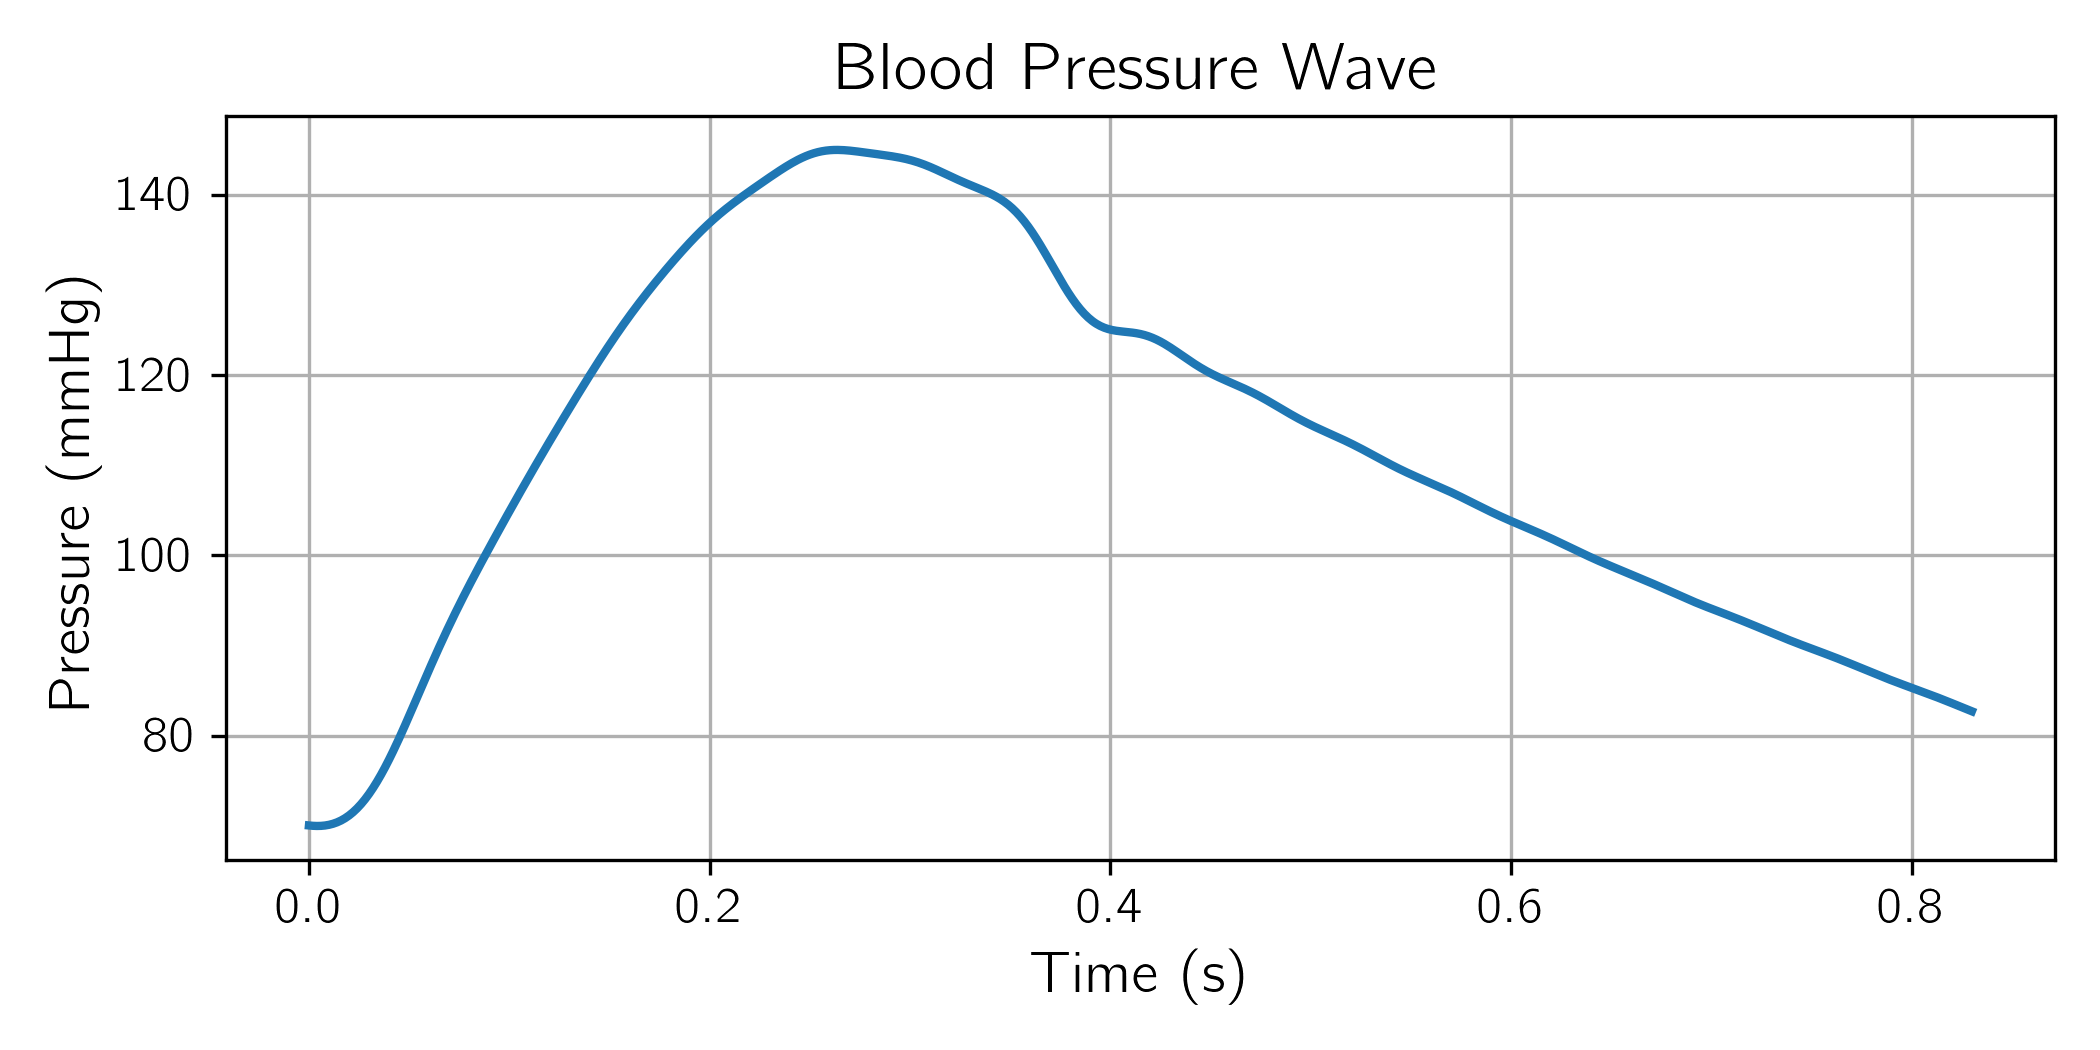
\includegraphics[width = 0.5\textwidth]{curve PW.png}
\caption{Incident blood Pressure Wave}\label{fig:BPW}
\end{figure}


\subsubsection{Results and discussion}
We again highly encourage watching the video's (\href{https://ugentbe-my.sharepoint.com/:f:/g/personal/constantijn_coppers_ugent_be/Evlx5Q0EKRhCggn-R1x3NKQBhiF82wRowFP4pT1nCn1ymg?e=Xi2V3R}{Biomedical application}), since they give more insight. Noteworthy;
\begin{enumerate}
\item we took the length of the BV (TL) to be $12$ m. That is only done to clarify the simulation and has no physical meaning; the pulse has a duration time of $1 \ \mathrm{s}$ so the PW 'fits' twice in the BV and a clear distinction before and after the reflection can be made.

\item The original pressure wave (Figure \ref{fig:BPW}) was scaled down such that the pressure drop $\Delta P$ in the BV is simulated. The basal blood pressure for this case is about 70 mmHg.

\item The parameters used to model the blood pressure pulse, are empirically deduced. Since we lack data and research about vasoconstriction and aneurysms, the values $R_L$ and $C_L$ are wisley chosen. 
\end{enumerate}

\begin{figure}[! h]
\centering
\begin{subfigure}{.5\textwidth}
  \centering
  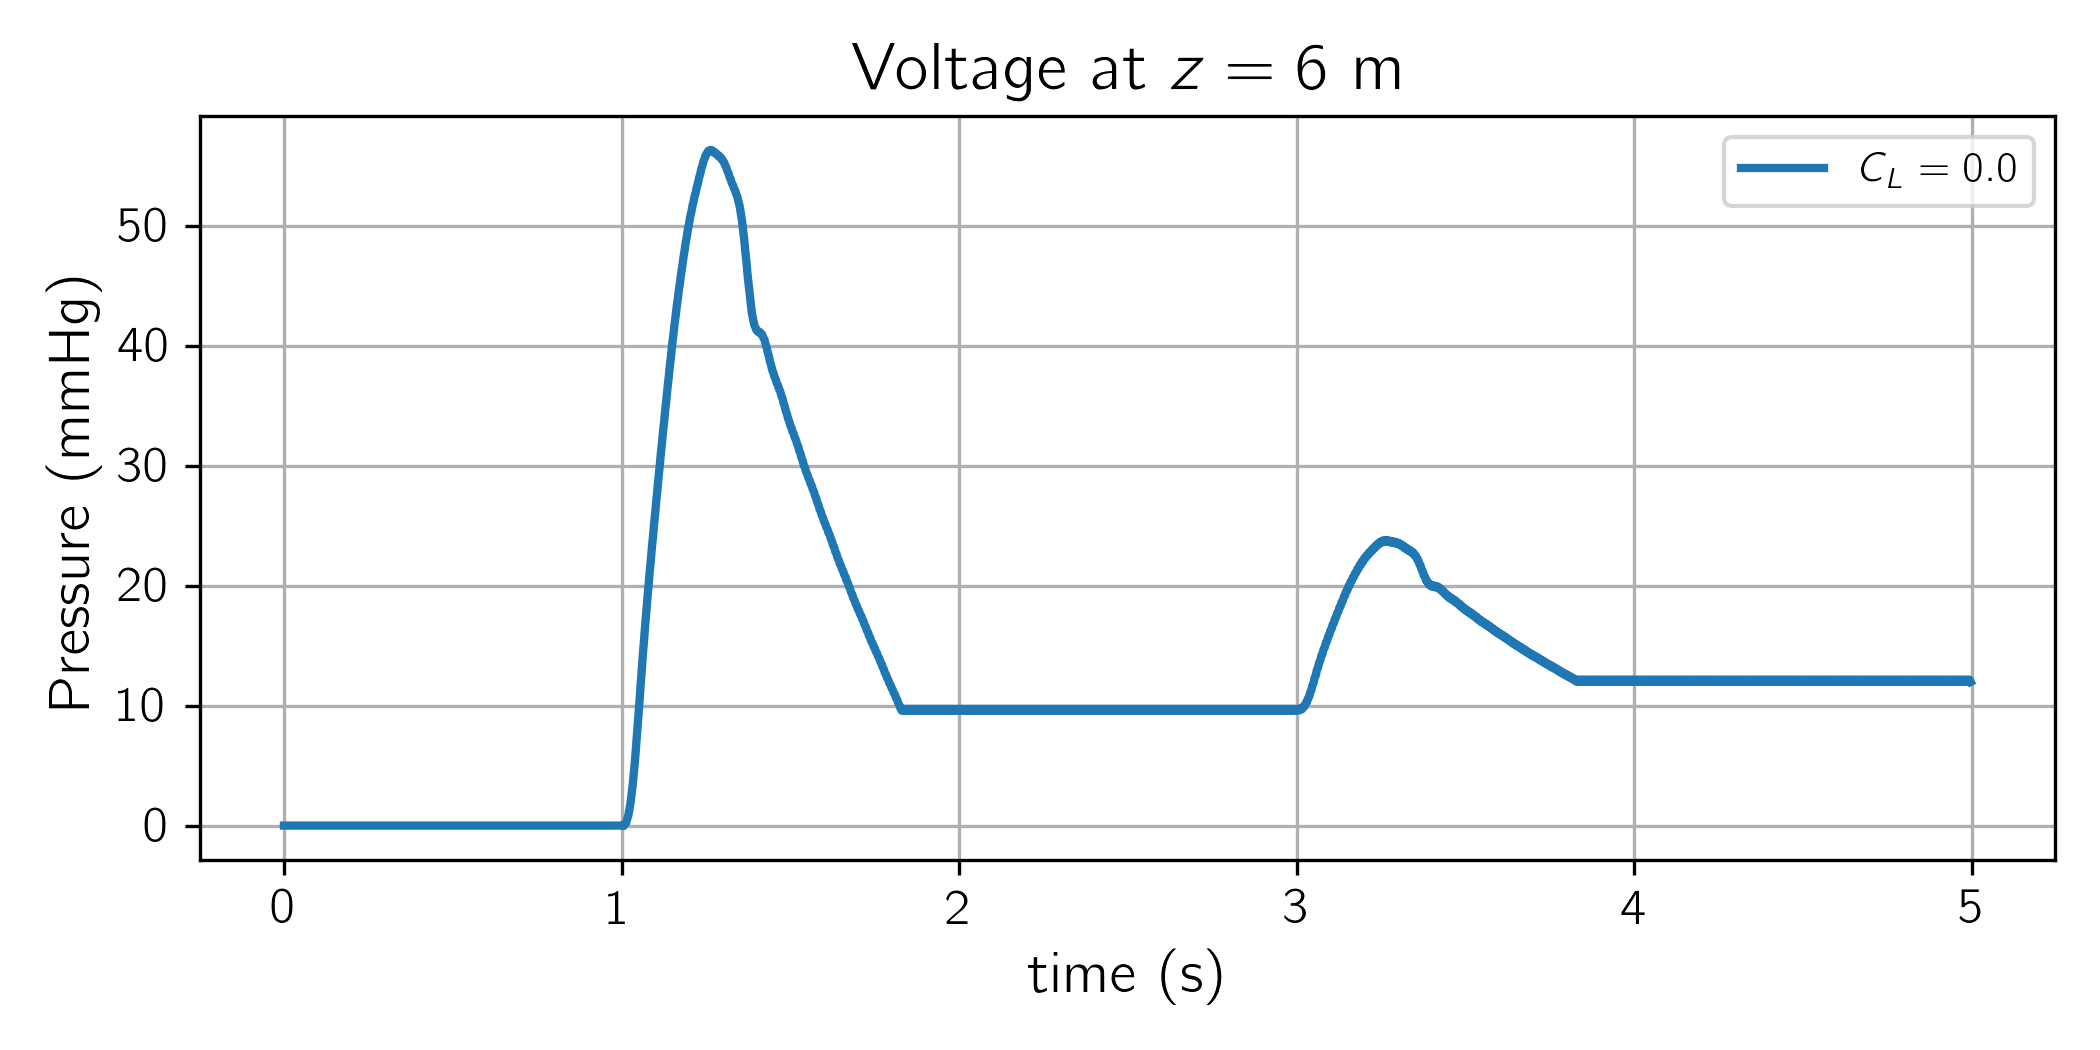
\includegraphics[width=\linewidth]{figures/PW_refl.png}
  \caption{Vasoconstriction}
  \label{fig:bv.refl}
\end{subfigure}%
\begin{subfigure}{.5\textwidth}
  \centering
  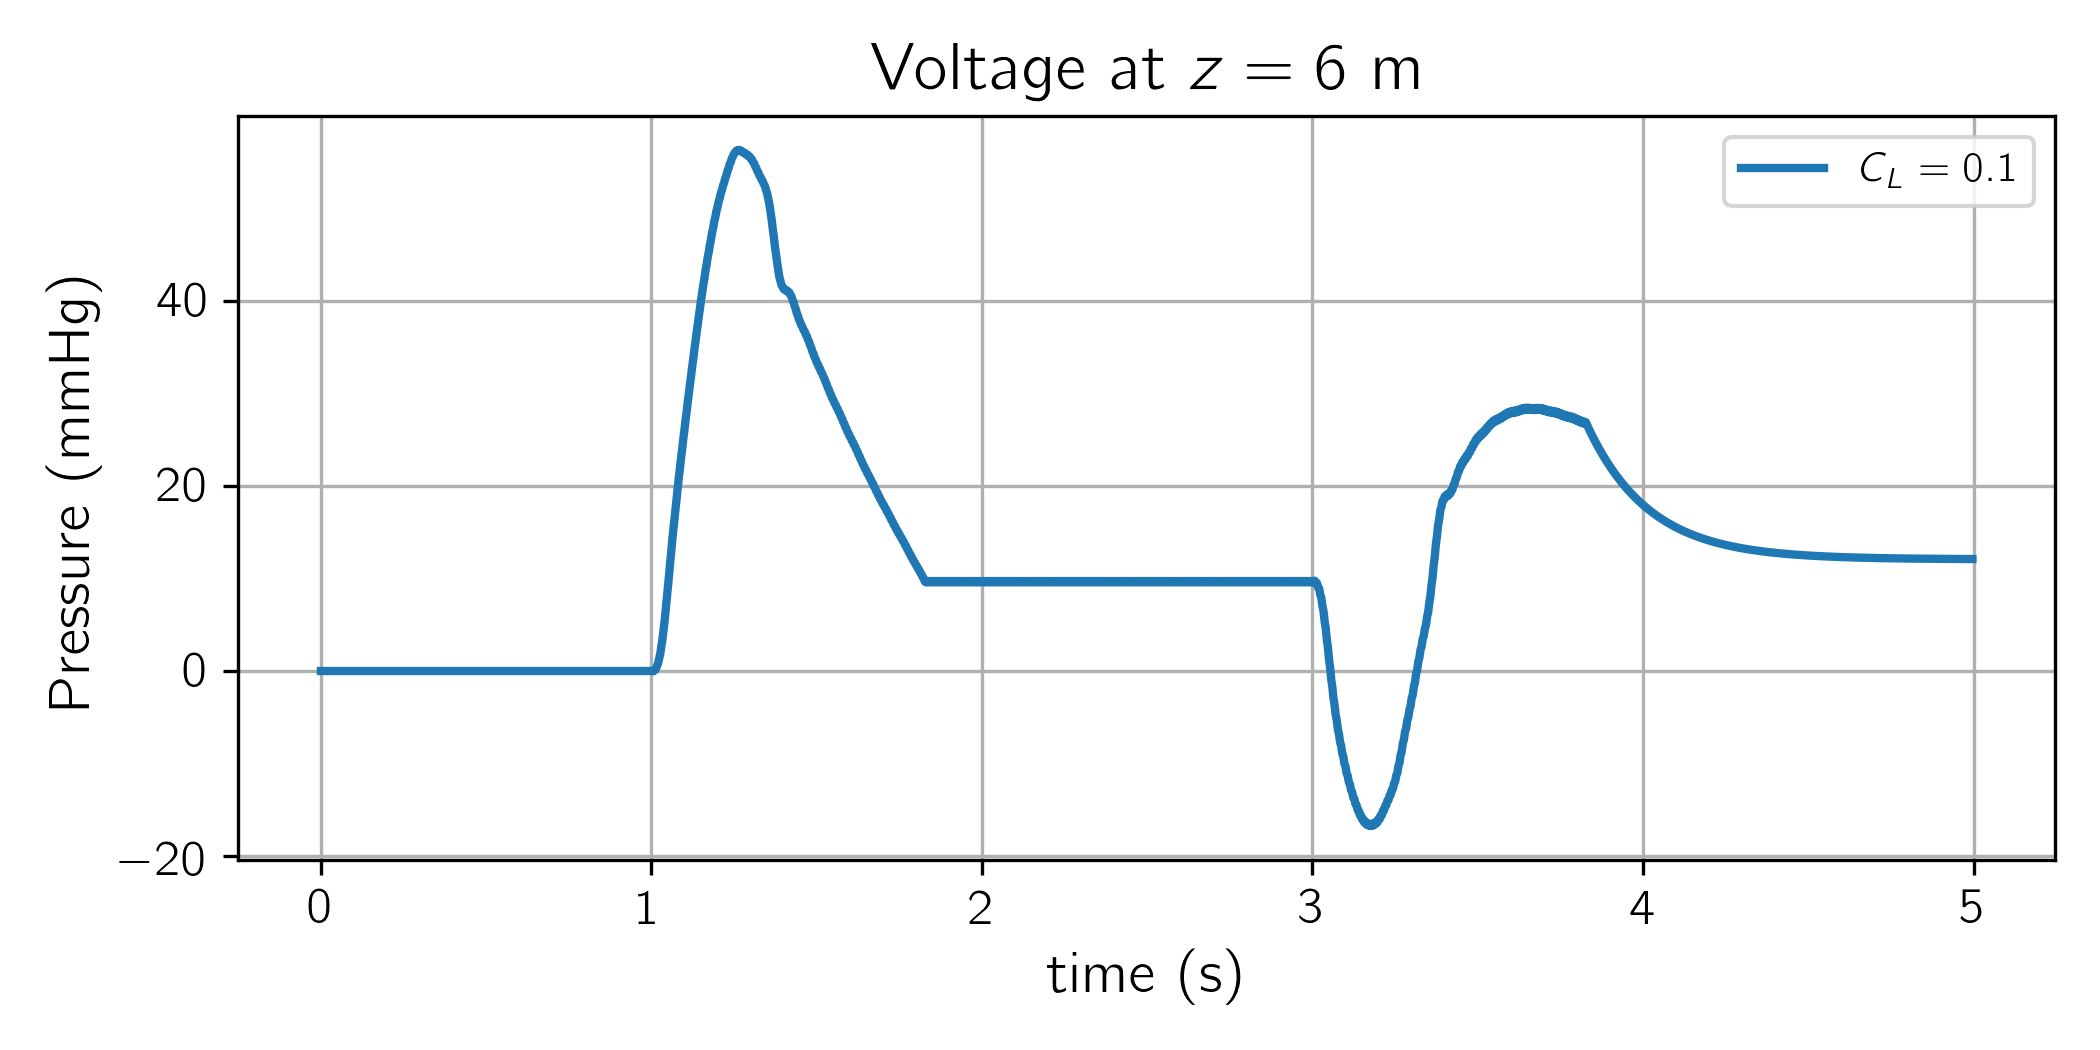
\includegraphics[width=\linewidth]{figures/PW_cap.png}
  \caption{Vasoconstriction in parallel with an aneurysm}
  \label{fig:bv.cap}
\end{subfigure}
\caption{Results of case 1 (a) and case 2 (b)}
\end{figure}

\subsubsection{Conclusion and future perspectives}
One can conclude that the LTL model is useful to predict how a PW will be reflected at a certain load. Especially since in vivo measurements are not easy obtainable. Nevertheless, This may be useful for cases with a relatively stiff, low branched BV's\footnote{e.g. reflection at a heart valve}. In contrary, The simulation is incomplete in many ways:
\begin{enumerate}
\item the used parameters are not representing the real values; there is a general difficulty in determining parameters that fit the pulse pressure wave as well as the load resistance and capacitance. Nowadays, these values are calculated from in vitro measurements;
\item BV's are highly elastic and thus lossless, hence the need for a lossy TL;
\item Silently, the BV diameter was assumed to be large enough. Blood is not newtonian; high shear stresses occur when the BV diameter approximates the size of blood cells;
\item Almost all BV are immensely branched; it is not easy to take this into consideration and model this.
\end{enumerate}

